\documentclass[french]{article}
\usepackage[T1]{fontenc}
\usepackage[utf8]{inputenc}
\usepackage{lmodern}
\usepackage[a4paper, margin=2.5cm]{geometry}
\usepackage{babel}
\usepackage[cache=false]{minted}
\usepackage{graphicx}
\usepackage{xcolor}
\usepackage{hyperref}
\definecolor{bg}{rgb}{0.98,0.98,0.98}

\title{Rapport Développement Logiciel}
\author{Badr YOUBI IDRISSI}

\begin{document}
	
\section{Introduction et fonctionnement général}

Dans ce projet nous codons un programme pour visualiser les isolignes 
d'un signal émit de plusieurs tétraèdres. Voici un schéma du fonctionnement
général :

\begin{center}
	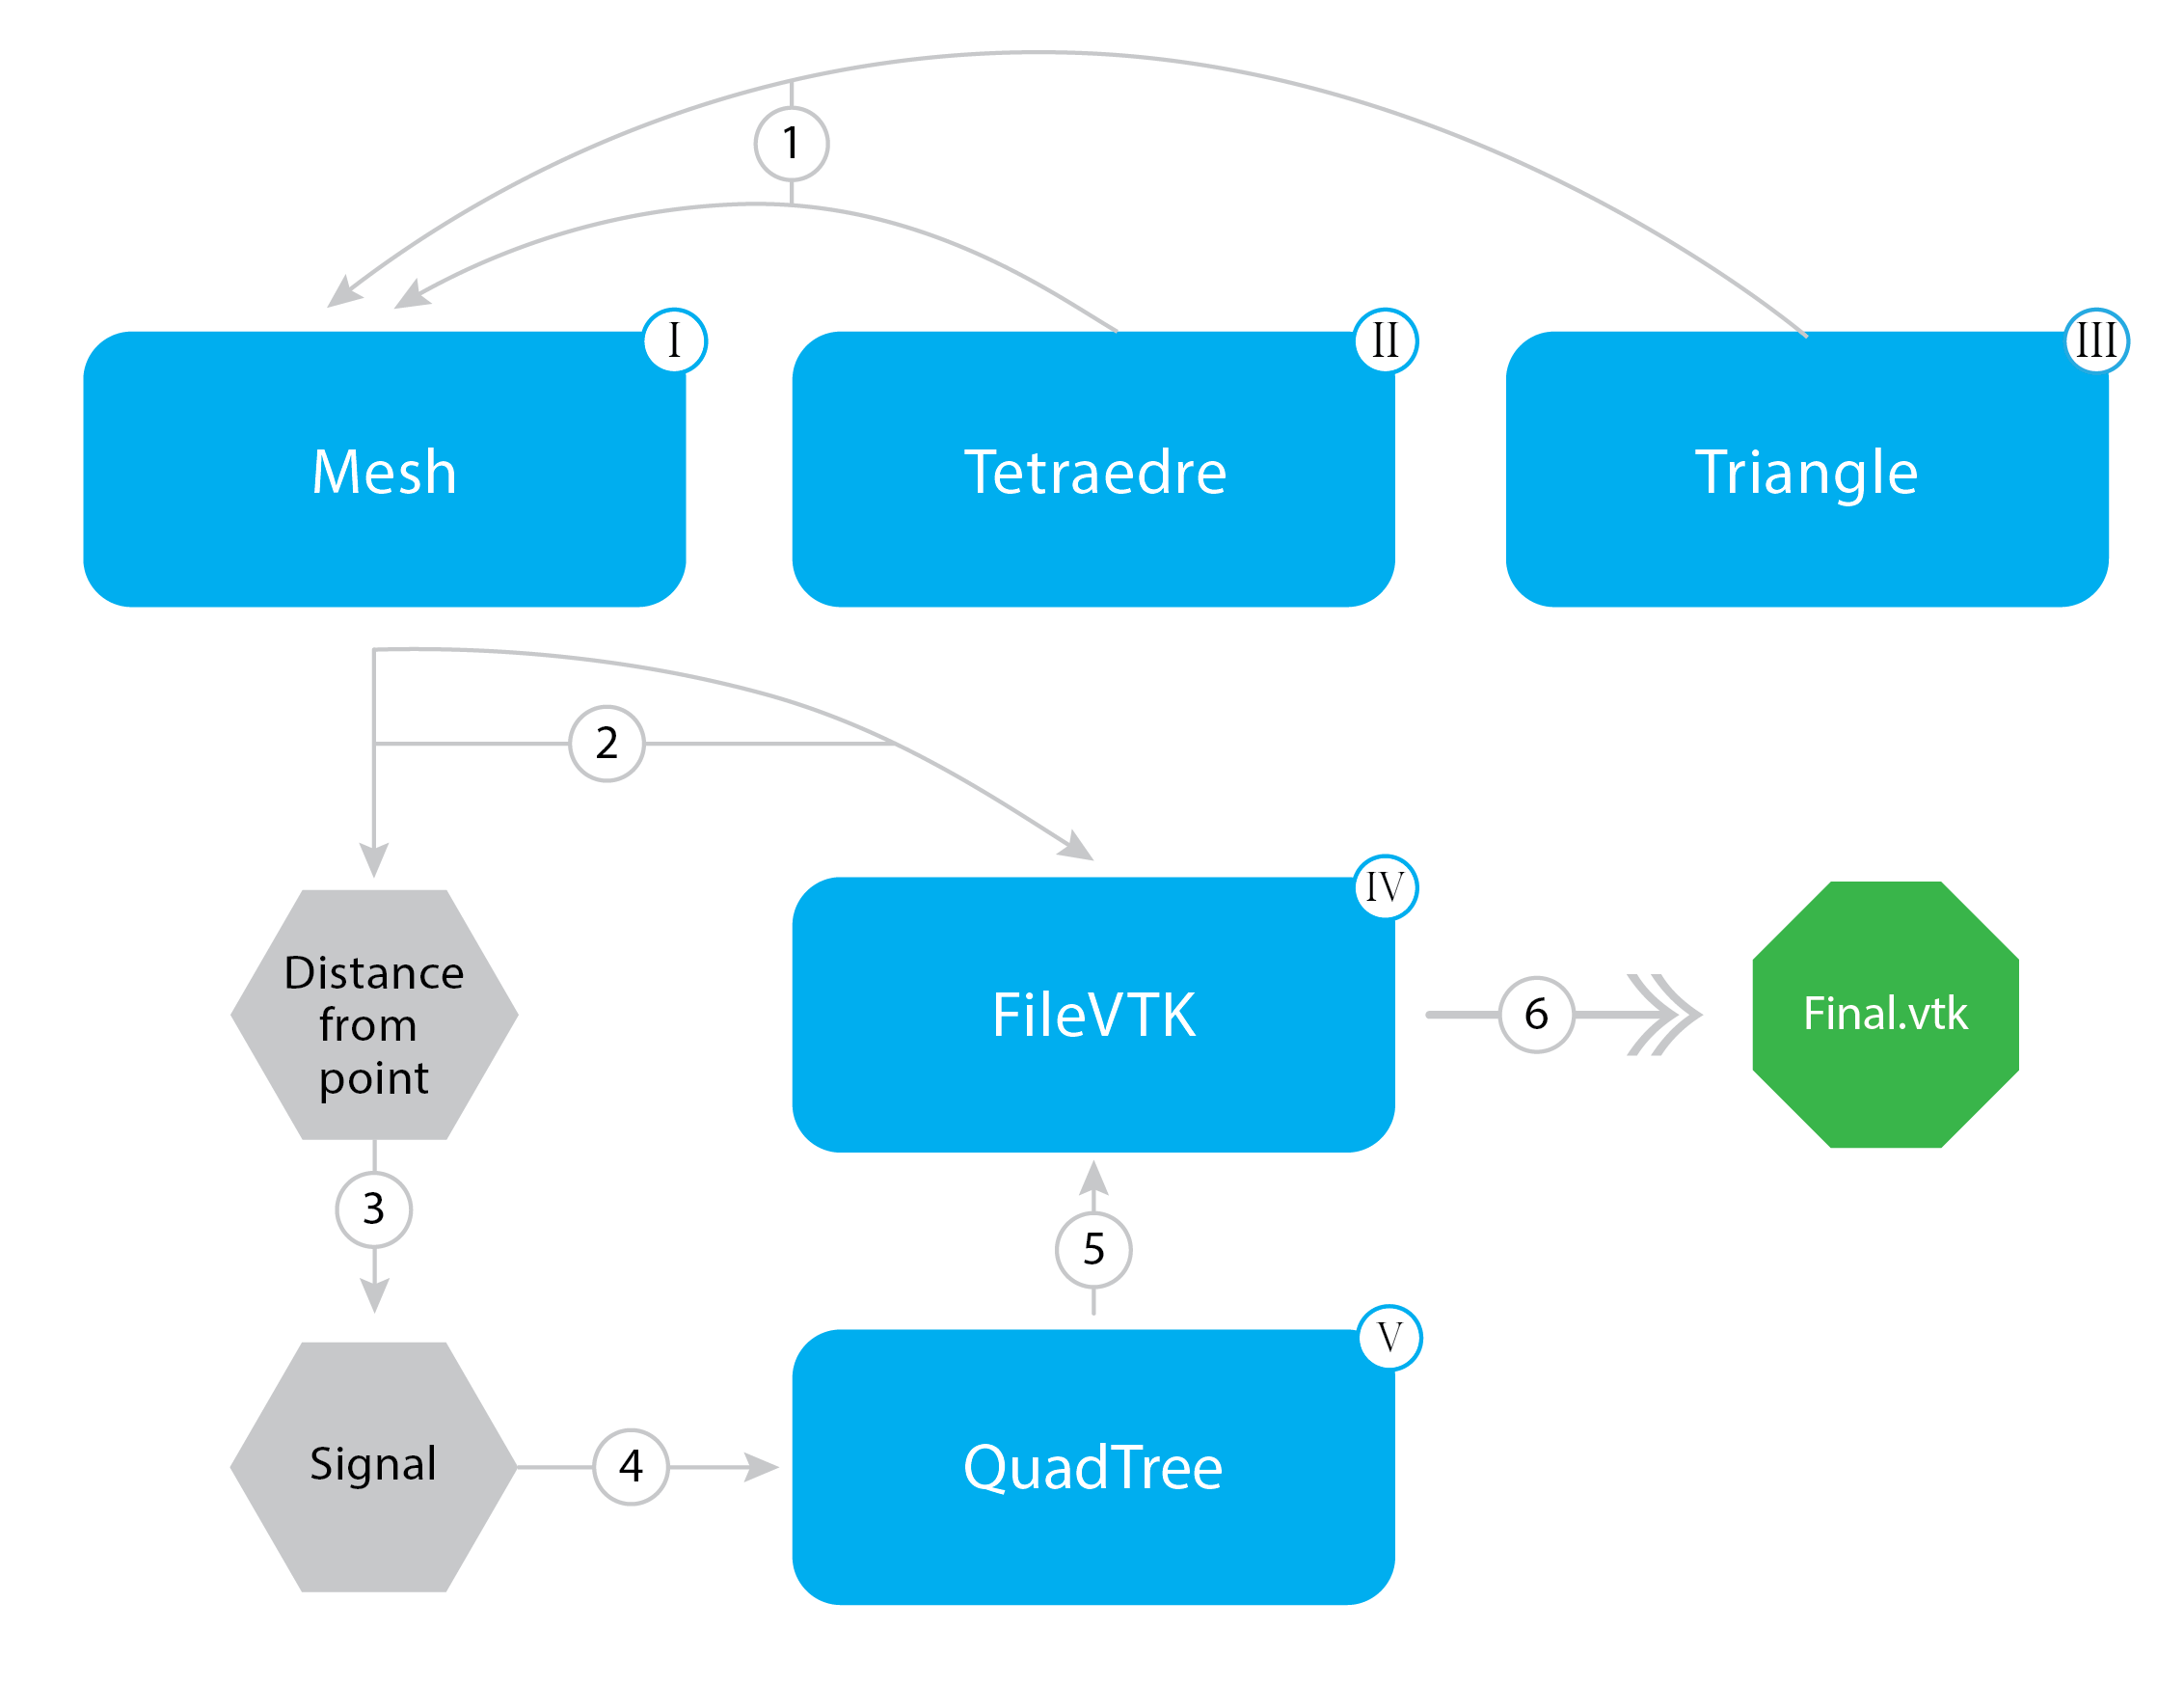
\includegraphics[width=0.7\textwidth]{Figures/SchemaNum.png}
\end{center}

On commence par créer l'objet 'Mesh' (\textit{I}) qui correspond à l'ensemble des pods émétant le signal.
L'objet mesh a besoin des points correspondant à chaque pod qui est un 'Tétraèdre' (\textit{II}) qui lui
même est un ensemble de 'Triangles' (\textit{III}) (\'Etape 1). Cet objet Mesh a la méthode distance from point qui 
renvoie la liste des distances entre un point et les pods (\'Etape 2). Ces distances servent ensuite à calculer le signal
en tout point de l'espace (\'Etape 3). on crée ensuite un plan à la hauteur 0.01 dont on va rafiner le maillage
avec l'objet 'QuadTree' (\textit{V}) (\'Etape 4). Ensuite l'ensemble des points et les valeurs du signal en ces points est
passé à l'objet 'FileVTK' (\textit{IV}) (\'Etape 5) qui va écrire le fichier "Final.vtk" (\'Etape 6).

\section{Description du code}
	
\subsection{Objet III : Triangle}
\vspace{10pt}
\begin{minted}[breakanywhere, xleftmargin=10pt]{python}

class tri:
	def __init__(self, point1, point2, point3): 
		...
	def distance_to_a_point(self, P): 
		...
\end{minted}

L'objet triangle sert à stocker les points du triangle et à calculer la distance entre
un point et à calculer la distance entre un point quelconque et le triangle.

\begin{minted}[breakanywhere, xleftmargin=10pt]{python}
def __init__(self, point1, point2, point3):
	self.points = [np.array(point1), np.array(point2), np.array(point3)]
	p1p2 = self.points[1]-self.points[0]
	p1p3 = self.points[2]-self.points[0]
	self.normal = np.cross(p1p2, p1p3)
	self.normal = self.normal/np.linalg.norm(self.normal)
\end{minted}
On enregistre les points A, B et C et on calcule la normale $ \overrightarrow{n'} = \overrightarrow{AB} \times \overrightarrow{AC} $
puis $ \vec{n} = \frac{\overrightarrow{n'}}{\|\overrightarrow{n'}\|}$

Pour la fonction de calcul de distance la fonction projète le point sur le plab du triangle puis selon 
les valeurs des coordonnées barycentriques on retourne la plus petite distance à un coin ou à un bord.
Au vu du grand nombre de cas, j'ai opté pour reprendre un code déjà fait qui applique ce principe 
(voir \href{run:https://gist.github.com/joshuashaffer/99d58e4ccbd37ca5d96e}{code})

\subsection{Objet II: Tetra}
\vspace{10pt}
\begin{minted}[breakanywhere, xleftmargin=10pt]{python}

class tetra:
	def __init__(self, point1, point2, point3, point4):
		...
	def distance_to_a_point(self, p):
		...

\end{minted}

L'objet tetra est un ensemble de triangles correctement orientés (normales vers l'extérieur) qui peut
calculer la distance entre un point et le tetra.
\begin{minted}[breakanywhere=true	, xleftmargin=10pt]{python}
def __init__(self, point1, point2, point3, point4):
	self.points = [point1, point2,point3,point4]
	self.faces = [tri(point1,point3,point2), tri(point1,point4,point3),
				 tri(point2,point3,point4), tri(point1,point2,point4)]
\end{minted}
L'ordre des points ici est important pour bien orienter les normales.


\end{document}
